\documentclass{report}
\usepackage[utf8]{inputenc}
\usepackage{amsmath}
\usepackage{amsfonts}
\usepackage{setspace}

\title{ Algebra and Analytic Geometry lecture }
\author{Philip Policki}
\date{9th October 2020}

%\usepackage{natbib}
\usepackage{graphicx}

\begin{document}
\graphicspath{{./imgs/}}
\maketitle
\tableofcontents
\pagebreak
\large
\chapter{Complex Numbers}
\section{Sets of numbers}
	\begin{itemize}
		\item Natural Numbers $N = \{1, 2, 3, 4, ...\}$
		\item Integers $Z = \{ ..., -3, -2, -1, 0, 1, 2, 3, ... \}$
		\item Rational Numbers $Q = \{  \frac{p}{q}; q,p \subset Z, q \neq 0  \}$
		\item Real Numbers $R \emph{Any distance from 0 on the number line}$
	\end{itemize}

\section{Operation law on numbers}

	\begin{enumerate}
	\item Commutative law \\ 
	$ a + b = b + a$ \\
	$ ab = ba $ 
	\item Associative law \\ 
	$ (a + b) + c = a + (b + c) $
	$ (ab)c = a(cb)$
	$ a(b+ c) = ab + bc $ 
	\end{enumerate}
For $\{N, Z, Q, R\}$ all the laws listed above are true 
\section{Divisibility}
	$A|B$  if there is a $c \subset N $
	
\section{Prime Numbers}
	A natural number $\neq 1$ is called a prime if it has only two divisors, namely 1 and itself. \\
	$Examples: 2, 3, 5, 7, ...$
	
	\subsection{Theorem}
	Every natural number can be uniquely (up to orders of factors) described as a product of prime numbers.\\
	$ Example: 24 = 2*2*2*3$

\section{Principle of Mathematical Induction}
Law for proving statements

If $ p_{1}, p_{2}, ..., p_{k} $ are statements and: 
	\begin{enumerate}
		\item $p_{1}$ is true
		\item if $p_{k}$ is true, then $p_{k + 1}$ is also true
	\end{enumerate}
Example: 

\section{Binomial formula}
Newtons formula for expanding powers of sums\\
$
(x+y)^1 = x + y \\
(x+y)^2 = x^2 + 2xy + y^2 \\ 
(x+y)^3 = x^3 + 3x^2y + 3xy^2 + x^2 \\
(x+y)^4 = \emph{To difficult to remember or to expand}
$

\subsection{Theorem}
$
(a + b)^n = \binom{n}{0}a^nb^0 + \binom{n}{1} a^{n-1}b^{1} + \binom{n}{2} a^{n-2}b^{2} + ... + \binom{n}{n} a^{n-n}b^{n}\\
$

This can be simplified to: \\
$
\sum\limits_{k=0}^n \binom{n}{k}a^{n-k}b^k
$

\subsection{Find a given coefficient of a given equation}
Question: Find the coefficient of $x^4$ in $(2x - \frac{1}{x})^6 \\ \\$
\\
$(2x - \frac{1}{x})^6 = (2x + \frac{-1}{x})^6 \\  \\
\sum\limits_{k=0}^6 \binom{6}{k}(2x)^{6-k}(\frac{-1}{x})^k 
$\\
To calculate 'k' to substitute it into the equation we have to have only one x so: \\
$
2^{6-k}x^{6-k}-x^{-k} -> x^{6-k-k} -> x^{6-2k}
$\\
Based on that and the fact that we want to get the coefficient of $x^4$ we do the following: \\
\\
$
6-2k = 4 \\
k = 1
$\\
So we substitute and we get: \\
\\
$\binom{6}{1}2x^{6-1} * (\frac{-1}{x})^1 = \frac{6!}{5!}2x^5 * \frac{-1}{x} =  6 * 2x^5  * \frac{-1}{x} = -12x^4 $ \\ 
\\
Therefore the answer is -12 


\section{Complex numbers}
Def: A complex number is a pair of real numbers.\\
Example: (2, 3) they are traditionally denoted by z, u, w .. . \\
The set of all complex numbers will be denoted by $\mathbb{C}$ so: \\
$\mathbb{C} = \{(x, y): x, y \in \mathbb{R} \}$ \\
if z = (x, y) $(x, y) \in \mathbb{R}$, then x is called the real part of z and denoted as $R_ez$ and y is the imaginary part.\\ \\
Geometric interpretation: \\
A complex number z=(x, y) can be viewed as a point on a Cartesian plane. Such plane will be called the complex plane. \\ \\
As Vectors on the plane with a initial point at the origin of the plane \\ \\

\subsection{Operations on complex numbers}
\begin{enumerate}
	\item Addition:\\ f $z_1 = (x_1, y_1)$, $z_2 = (x_2, y_2) \in \mathbb{C}$, then their sum is defined to be $z_1 + z_2 = (x_1 + x_2, y_1 + y_2)$ \\
	$(1, 0)+(b, 0) = (a+b, 0)$
	\item Multiplication:\\ if $z_1 = (x_1, y_1), z_2 = (x_1, y_1)$ then their product is defined to be the number $z_1z_2=(x_1x_2 - y_1y_2,\; x_1y_2 + x_2y_1)$ \\
	Example: $(1,2)*(3, -1) = (1*3 - 2(-1), \; 1(-1), 3*2) = (5, 5)$ \\
	Properties: Commutative and Associative \\
	$(a, 0)(b, 0) = (ab, 0)$ \\
	$(0, 1)(0, 1) = (-1, 0)$\ \\
	$z = (x,y) = (x, 0) + (0, y) = (x, 0) + (0, 1)(y, 0) = x+iy$
	\item Better multiplication: \\
	$(3 + 2i)(1 - 2i) = (3+2i)1 + (3+2i)(2i) = 3+2i+6i-4=-1 + 8i$
	\item Inverse: \\
	$z = x+ iy$ \\
	$w = \frac{x}{x^2 + y^2} = i\frac{-y}{x^2 + y^2}$ \\ 
	$w = \frac{1}{z}$ 	
	\item Conjugate: \\
	Properties: \\
	$\overline{z} = x+i(-y) = x-iy$
	\begin{enumerate}
		\item $\overline{z+w} = \overline{z} + \overline{w}$
		\item $\overline{z*w} = \overline{z} * \overline{w}$
		\item $\overline{z^n} = \overline{z}^n$
	\end{enumerate}
	\pagebreak
	\item Modulus: \\
	if $z=x+iy$ the modulus is $|z|=\sqrt{x^2 + y^2}$
	Properties: \\
	\begin{itemize}
		\item $|z| \geq 0$ and $|z|=0 \equiv z=0$
		\item $|\bar{z}| = |z|$
		\item $|zw| = |z|*|w|$
		\item $|z^n| = |z|^n$   $n\in\mathbb{N}$
		\item $|z+w| \leq |z| + |w|$
		\item $z\bar{z} = |z|^2$
	\end{itemize}
\end{enumerate}
\subsection{Polar form}
A polar form of a complex number $z\neq 0$ is the form $z=r(\cos(\alpha) + i\sin(\alpha))$, where $r>0$
Example: \\
\setstretch{1.2}
\LARGE
$z = 3(\cos(\frac{\pi}{2}) + i\sin(\frac{\pi}{2}))$ \\
\large
If $z=r(\cos\alpha + i\sin\alpha), \; w=rR(\cos\alpha + i\sin\alpha)$\\
\begin{itemize}
	\item $zw = rR[\cos(\alpha + \beta) + i\sin(\alpha + \beta)]$
	\item $\frac{z}{w} = \frac{r}{R}[\cos(\alpha - \beta) + i\sin(\alpha - \beta)]$
	\item $z^n = r^n [\cos(n\alpha) + i\sin(n\alpha)]$
\end{itemize}
\pagebreak
\subsection{Geometry of algebra of complex numbers}
\begin{figure}[h!]
	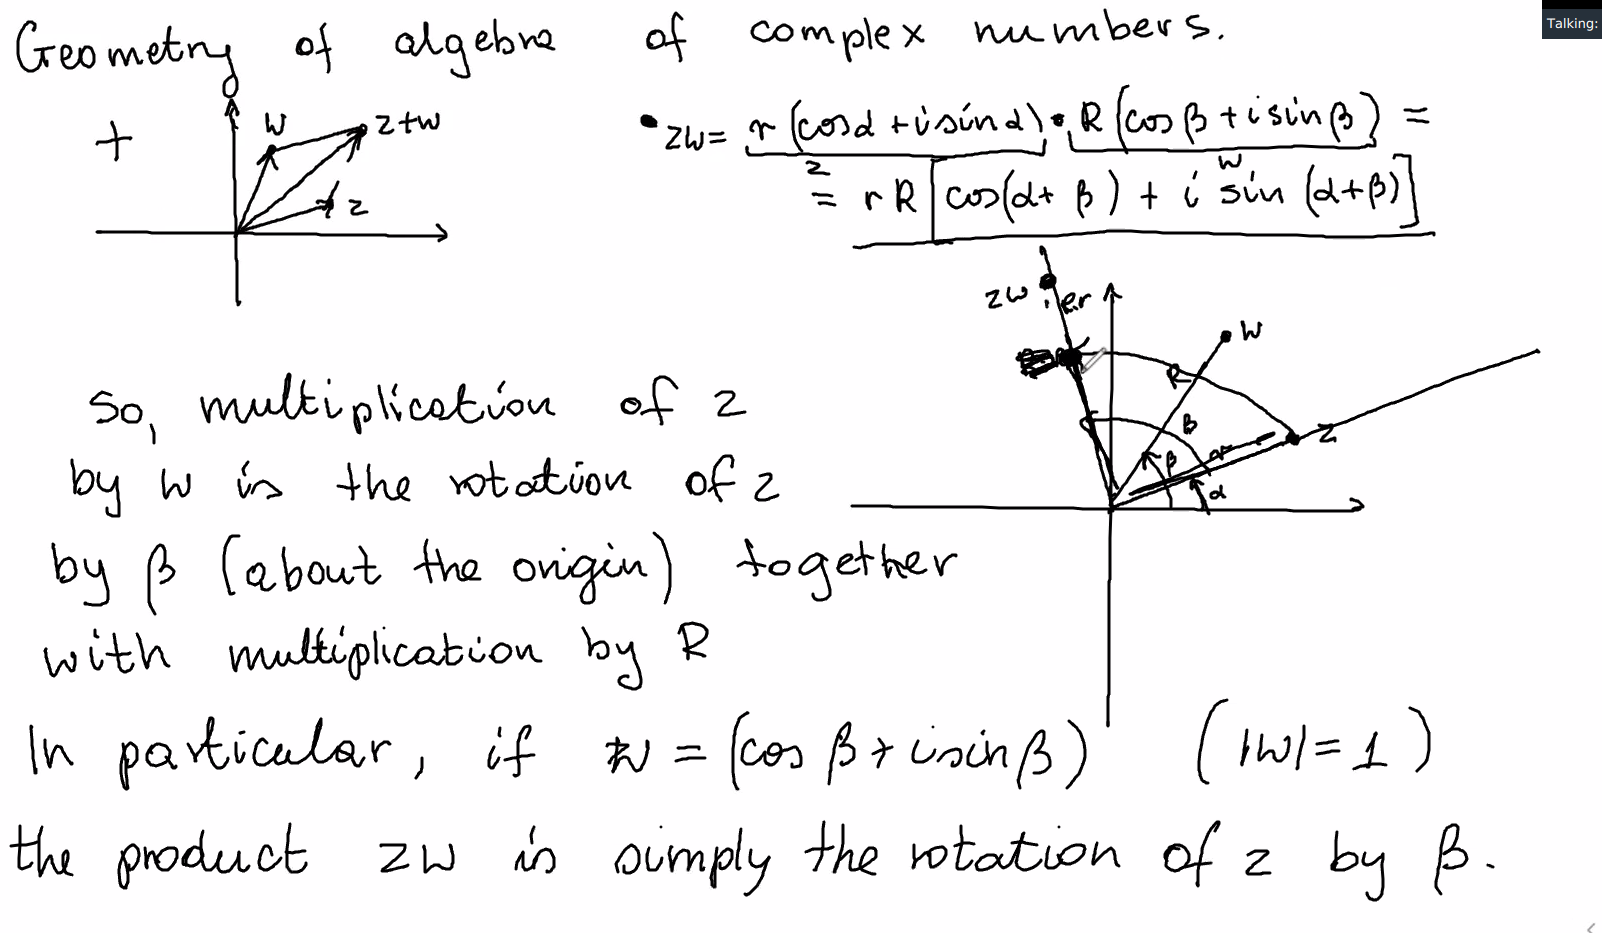
\includegraphics[scale=0.25]{algebra-lecture1.png}
	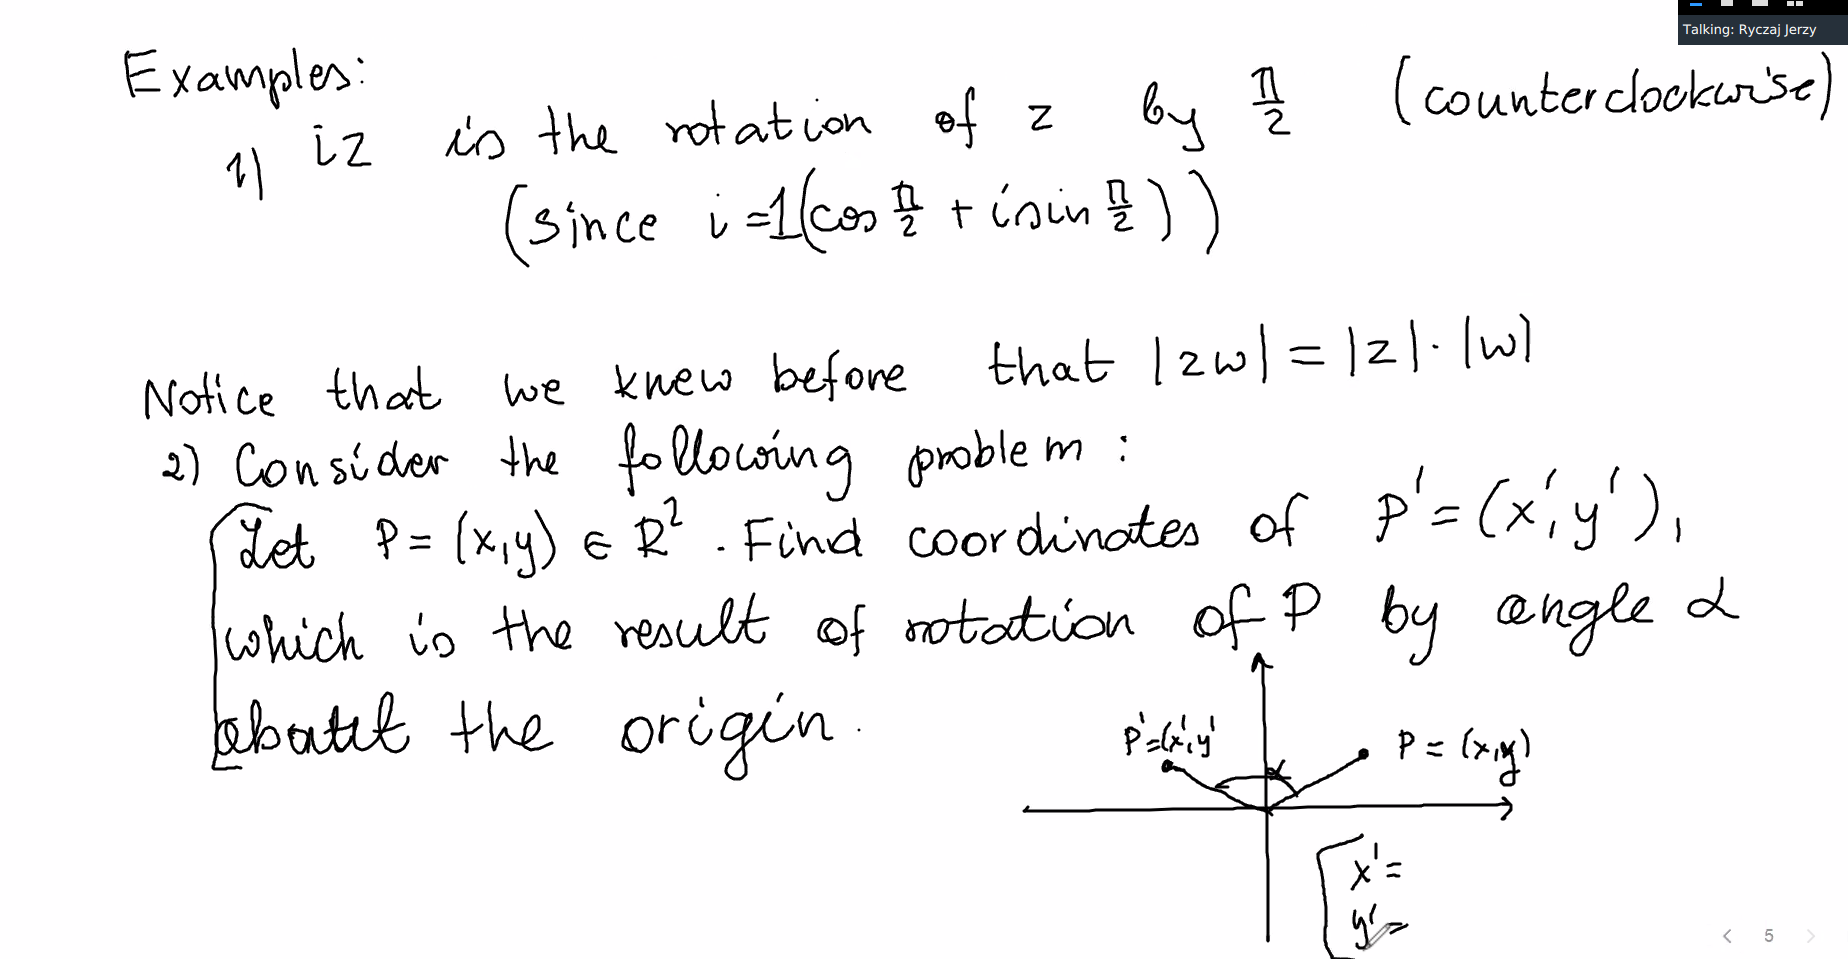
\includegraphics[scale=0.25]{2.png}
	\centering
\end{figure}
\subsection{Roots}
Consider equation $z^n = W$. \\
The $n^{th}$ root of a complex number w is the set $\{z: z^n=w\}$. We denote it by $\sqrt[n]{w}$.
Properties: 
\begin{itemize}
	\item If $w=0$, then $\sqrt[n]{0} = \{0\}$
	\item if $w\neq 0$, then $\sqrt[n]{0}$ has exactly n elements
\end{itemize}
Examples: 
\begin{itemize}
	\item $\sqrt{-1} = \{i, -i\}$
	\item $\sqrt{4}^{(\mathbb{C})} = \{2, -2\}$ it may be a real or complex root
\end{itemize}
If $w = r(\cos\alpha + i\sin\alpha)$, then $z^n=w$ has exactly  n solutions given by 
$z_k = \sqrt[n]{r}[\cos(\frac{\alpha + 2k\pi}{n}) + i\sin(\frac{\alpha + 2k\pi}{k})]$.


\section{Polynomials}
A (complex) polynomial is a function of the form: $W(z) = a_0 + a_1z + ... + a_nz^n$, where $a_0, a_1, ..., a_n \in\mathbb{C}$ and are called coefficients. \\
A degree of a nonzero polynomial is the largest n such that $a_n \neq 0$. For zero polynomial $W(z) = 0$ we agree that its degree is $-\infty$. \\
Examples:
\begin{enumerate}
	\item $W(z) = (i+2)z^2 + z -i$
	\item $W(z) = i + z^3$
\end{enumerate}
If $a_0, a_1, ..., a_n \in\mathbb{R}$, then W(z) is called a real polynomial. We can add and multiply polynomials as functions. Moreover if $W_1, W_2, W_3$ are polynomials, then
\begin{itemize}
	\item $W_1 + W_2 = W_2 + W_1$
	\item $(W_1 + W_2) + W_3 = W_1 + (W_2 + W_3)$
	\item $W_1W_2 = W_2W_1$
	\item $W_1(W_2W_3) = (W_1W_2)W_3 = W_1W_2W_3$
	\item $W_1(W_2 + W_3) = W_1W_2 + W_1W_3$
\end{itemize}
We can always divide two polynomials: $W(Z) : P(Z) = Q(z)$. If $W(Z), P(Z)$ are polynomials, then there are polynomials $Q(Z), R(Z)$ such  that $W(Z) = P(Z)Q(Z) + R(Z)$ \\ \\
A complex number $z_0$ is a root of a polynomial $W(Z)$ if $W(z_0) = 0$.\\ \\
\subsection{Bezout Theorem}
$z_0$ is a root of $W(z)\Leftrightarrow W(z)$  is divisible by $z_0$ \\ \\
\subsection{Fundamental Theorem of Algebra}
Every polynomial of degree $\geq$ 1 has at least one complex root. If $W(z)$ is a polynomial of degree $n\geq 1$, then there are complex numbers $z_1, z_2, ..., z_n$ such that $W(z) = A(z-z_1)(z-z_2) ... (z-z_n)$



\subsection{Rational Functions}
A rational function is a function of the form $f(x) = \frac{P(x)}{Q(x)}$, where P, Q are polynomials. \\
$f(x) = \frac{4x^2 - x + 2}{x-3ix^3}$.\\
If both P(x), Q(x) are real polynomials, then $f(x) = \frac{P(x)}{Q(x)}$ is called a \underline{real rational function}.\\
A rational function $f(x) = \frac{P(x)}{Q(x)}$ is called a \underline{proper rational function} if the degP $<$ degQ.\\

\subsubsection{Theorem}
If $f(x) = \frac{P(x)}{Q(x)}$ is a rational function, then it can be written as a sum of a polynomial and a proper rational function. \\
Every real rational function is a sum of a real polynomial and a real proper rational function.



\subsubsection{Partial Fraction}
A partial fraction is a (proper) rational function of the form:
\Large
\begin{itemize}
	\item $\frac{A}{(x-a)^n}$, $A\in\mathbb{R}$, $n\in\mathbb{N}$ 1st type
	\item $\frac{Ax + B}{(ax^2 + bx  + c)^m}$, $A,B,a,b,c\in\mathbb{R}$, $m\in\mathbb{N}$ 2nd Type
\end{itemize}
\large


\subsubsection{Partial fractions decomposition}
Every proper rational function can be written as a sum of partial fractions. Moreover if $\frac{P(x)}{Q(x)}$ is a proper rational function then
\begin{itemize}
	\item If $(x-a)^n$ is a factor of $Q(x)$ and $(x-a)^{n+1}$ is not, then in partial fractions decomposition we will get terms, $\frac{A_1}{(x-a)^1}$, $\frac{A_2}{(x-a)^2}$, ..., $\frac{A_n}{(x-a)^n}$
	\item If $ax^2 + bx + c$ with $\Delta < 0$ appears in decomposition of $Q(x)$ exactly n times
	\item No other terms will appear in the decomposition of $\frac{P(x)}{Q(x)}$
\end{itemize}
\LARGE
If $W_1(x) = a_0, a_1x + ... + a_nx^n$, $W_2(x) = b_0, b_1x + ... + b_nx^n$, then $W_1 = W_2 \leftrightarrow \\ \forall_{x\in\mathbb{R}} W_1(x) = W_2(x) \leftrightarrow \\ \forall_{k=0, 1, 2, ... , n} a_k = b_k \leftrightarrow \\ \forall_{z\in\mathbb{C}} W_1(z) = W_2(x)$
\large



\chapter{Matrices}

\section{Algebra of Matrices}
A matrix is an array consisting of numbers (real or complex). The whole theory is identical foe both real and complex numbers. We will develop it in case of real numbers. Elements of a matrix are called entries. If a matrix consist of m rows and n columns than we say that it is of size m x n. \\
Matrices 1 x 2 can be identified with points on a plane (with coordinate system)

\subsection{Special Types of Matrices}
\begin{enumerate}
	\item Zero matrices will be denoted by 0
	\item Square matrices, they have size of n x n
\end{enumerate}

\section{Kronecker-Capelli Theorem}
A system $AX = B$ has a solution $ \Leftrightarrow $ rank(A) = rank([$A | B$]) \\
Moreover if the system has m equations in n variables, then if 
\begin{enumerate}
	\item rank(A) = rank([$A | B$]) = n, then the system AX = B has a unique solution
	\item rank(A) = rank([$A | B$]) < n, then the system AX = B has an infinite number of solutions, depending on n-k parameters.
\end{enumerate}


\chapter{Analytic Geometry}
$R^n$ is a set of {($x_1, x_2, x_n$)!, $x_1, ..., x_n \in\mathbb{R}$}. Elements of $R^n$ will be called vectors and we will denote them by $\vec{u}$, $\vec{w}$

\section{Geometric interpretation}
\begin{enumerate}
	\item $R^1$ can be interpreted as points on a line
	\item $R^2$ can be interpreted as vectors or points on a plane
	\item $R^3$ can be interpreted as vectors in 3d space
\end{enumerate}

\section{Operations in $R^n$}
\begin{enumerate}
	\item Vector addition same as in matrices
	\item Multiplication by a number same as in matrices
	\item Dot product $\vec{u} \circ \vec{v} = x_1y_1 + x_2y_2 + ... + x_ny_n$
\end{enumerate}

\section{Operations in $R^3$}
\begin{enumerate}
	\item $\vec{u} * \vec{u} = (y_1z_2 - y_2z_1, -(x_1z_2 - x_2z_1), x_1y_2-x_2y_1)$
\end{enumerate}
\end{document}